\chapter{SCOBY Machine \& Materials}


\section{Overview}

In the same way as for the environent control project with the scoby, we had to think about how machines can help us make this new material our own, in much the same way as 3D printers popularized the use of PLA. 

The methods and machines presented here are designed to facilitate the use of this biomaterial, with the aim of optimizing the production of bacterial cellulose and changing the growing conditions to produce 3D cellulose. 

In addition, unlike mycelium, which unfolds in a substrate contained in a mold, cellulose requires more attention to shape channelling, both for molding and demolding. 

% \begin{figure}[h]
%     \centering
%     \includegraphics{images/Myceliummachine.png}
%     \caption{System design representation}
%     \label{fig:}
% \end{figure} 

\section{Systems design}


In the traditional approach, cellulose grows on the surface of the liquid, which means that the cellulose takes on a flat shape \- the shape of the container in which the bacterial cellulose grows. 

With the bioreactor, there are two objectives. on the one hand, to optimize production. On the other hand, to modify the natural growth of poccesus in order to be able to make more complex shapes than 2D shapes. 

To achieve this, the method used is to introduce a 3D shape that rotates on the surface of the liquid so that the cellulose can adhere to the shape and push against it. As shown in the following diagram. 

the bioreactor incorporates a rotating framework, typically shaped to encourage cellulose attachment and buildup in desired forms beyond a simple flat surface. This framework is submerged in a controlled culture medium, allowing the bacteria to deposit cellulose around a defined 3D scaffold as it rotates. The rotation ensures even cellulose distribution, encouraging layers to adhere around the object and gradually form into three-dimensional shapes.
\begin{figure}[h]
    \centering
    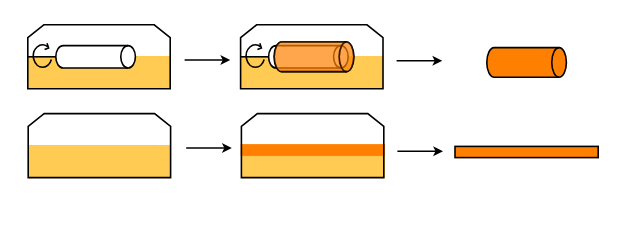
\includegraphics{images/shema3Dscoby.png}
    \caption{System design representation for 3D bacterial cellulose}
    \label{fig:diagBC3D}
\end{figure} 

The bioreactor takes the form of a closed space like a box, with openings covered with microporous plaster to allow air to pass through without contaminating the space. Into which the culture medium can be introduced.
It is generally located in a closed space in which a heating mat is installed to maintain a suitable temperature for better cellulose development. 
heating mat helps sustain an optimal temperature for bacterial activity, while microporous openings enable airflow, preventing contamination while ensuring that the bacteria have sufficient oxygen. Adjusting rotation speed and environmental factors enables control over cellulose thickness.


\section{Manufacturing Processes \& Grow Theory}


\begin{figure}[h]
    \centering
    \includegraphics{images/prodperso.png}
    \caption{Bacterial cellulose after growth period}
    \label{fig:manufactureperso}
\end{figure} 
In kombucha production, bacterial cellulose naturally forms a film on the surface of the liquid medium. The Acetobacter bacteria in the SCOBY (Symbiotic Culture of Bacteria and Yeast) convert sugars in the medium into long cellulose fibers when exposed to oxygen. This fibrous structure gradually accumulates, forming a thick cellulose layer that acts as a barrier, potentially preventing other microorganisms from entering the medium. The cellulose matrix produced this way is thought to provide protection for the bacteria by limiting microbial competition.

This cellulose production process operates from the top of the solution downward. As cellulose accumulates, the older layers sink, leaving the most recently formed cellulose on the top surface exposed to oxygen. This layered formation is key to producing thick, multi-layered sheets of cellulose that can later be harvested.

The process of creating bacterial cellulose involves two main stages: preparing the culture medium and setting up the bioreactor. In preparing a homemade culture medium, freshly crushed bacterial cellulose is added to a nutrient solution composed of tea, water, sugar, and a small amount of vinegar to maintain an acidic environment conducive to bacterial growth.

\-- Boil the Water: This step sterilizes the water and allows the tea to fully infuse.
\-- Add Tea, Sugar, and Vinegar: These elements provide essential nutrients. The tea provides nitrogen, while sugar is the primary energy source for the bacteria. Vinegar lowers the pH, creating a favorable acidic environment.
\-- Cool the Solution: Allow the mixture to cool below 30°C to avoid harming the living cultures.
\-- Introduce Crushed Cellulose: Adding bacterial cellulose from an older culture introduces live bacterial strains to kickstart the cellulose production.

Once the medium is prepared, it is transferred into a bioreactor, typically a container that promotes even growth. After approximately 14 days, a cellulose mat forms on the surface. This mat is then harvested, and the process can be repeated to cultivate a cellulose strain optimized for desired growth characteristics.

Drying and Final Processing: After growth, the cellulose mat is carefully removed and dried to achieve its final texture and strength. The drying process removes about 90\% of its water content, reducing the cellulose sheet to its final shape and thickness, making it durable and ready for various applications.


\begin{figure}[h]
    \centering
    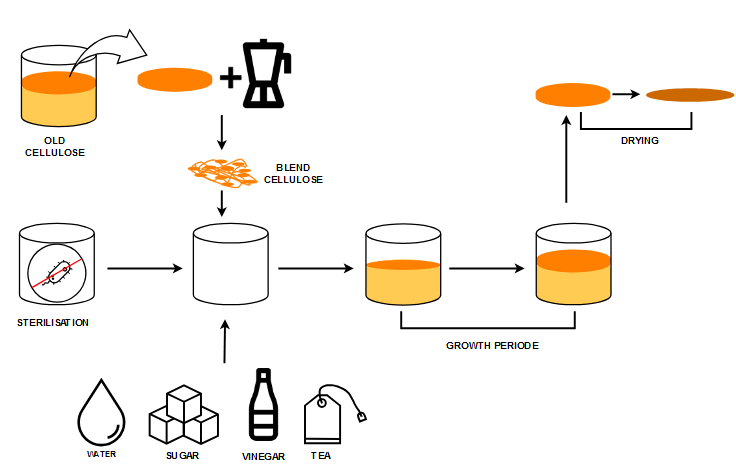
\includegraphics[width=1.4\textwidth]{images/SCOBY_diag.png}
    \caption{Classical manufacturing processes}
    \label{fig:manufacture}
\end{figure} 

\section{Contribution}

\subsection{Rotary Bioreactor}


\section{Result}

